\documentclass[11pt,compress,t,notes=noshow, xcolor=table]{beamer}
\documentclass[11pt,compress,t,notes=noshow, xcolor=table]{beamer}
\usepackage[]{graphicx}\usepackage[]{color}
% maxwidth is the original width if it is less than linewidth
% otherwise use linewidth (to make sure the graphics do not exceed the margin)
\makeatletter
\def\maxwidth{ %
  \ifdim\Gin@nat@width>\linewidth
    \linewidth
  \else
    \Gin@nat@width
  \fi
}
\makeatother

\definecolor{fgcolor}{rgb}{0.345, 0.345, 0.345}
\newcommand{\hlnum}[1]{\textcolor[rgb]{0.686,0.059,0.569}{#1}}%
\newcommand{\hlstr}[1]{\textcolor[rgb]{0.192,0.494,0.8}{#1}}%
\newcommand{\hlcom}[1]{\textcolor[rgb]{0.678,0.584,0.686}{\textit{#1}}}%
\newcommand{\hlopt}[1]{\textcolor[rgb]{0,0,0}{#1}}%
\newcommand{\hlstd}[1]{\textcolor[rgb]{0.345,0.345,0.345}{#1}}%
\newcommand{\hlkwa}[1]{\textcolor[rgb]{0.161,0.373,0.58}{\textbf{#1}}}%
\newcommand{\hlkwb}[1]{\textcolor[rgb]{0.69,0.353,0.396}{#1}}%
\newcommand{\hlkwc}[1]{\textcolor[rgb]{0.333,0.667,0.333}{#1}}%
\newcommand{\hlkwd}[1]{\textcolor[rgb]{0.737,0.353,0.396}{\textbf{#1}}}%
\let\hlipl\hlkwb

\usepackage{framed}
\makeatletter
\newenvironment{kframe}{%
 \def\at@end@of@kframe{}%
 \ifinner\ifhmode%
  \def\at@end@of@kframe{\end{minipage}}%
  \begin{minipage}{\columnwidth}%
 \fi\fi%
 \def\FrameCommand##1{\hskip\@totalleftmargin \hskip-\fboxsep
 \colorbox{shadecolor}{##1}\hskip-\fboxsep
     % There is no \\@totalrightmargin, so:
     \hskip-\linewidth \hskip-\@totalleftmargin \hskip\columnwidth}%
 \MakeFramed {\advance\hsize-\width
   \@totalleftmargin\z@ \linewidth\hsize
   \@setminipage}}%
 {\par\unskip\endMakeFramed%
 \at@end@of@kframe}
\makeatother

\definecolor{shadecolor}{rgb}{.97, .97, .97}
\definecolor{messagecolor}{rgb}{0, 0, 0}
\definecolor{warningcolor}{rgb}{1, 0, 1}
\definecolor{errorcolor}{rgb}{1, 0, 0}
\newenvironment{knitrout}{}{} % an empty environment to be redefined in TeX

\usepackage{alltt}
\newcommand{\SweaveOpts}[1]{}  % do not interfere with LaTeX
\newcommand{\SweaveInput}[1]{} % because they are not real TeX commands
\newcommand{\Sexpr}[1]{}       % will only be parsed by R
\newcommand{\xmark}{\ding{55}}%


\usepackage[english]{babel}
\usepackage[utf8]{inputenc}

\usepackage{dsfont}
\usepackage{verbatim}
\usepackage{amsmath}
\usepackage{amsfonts}
\usepackage{amssymb}
\usepackage{bm}
\usepackage{csquotes}
\usepackage{multirow}
\usepackage{longtable}
\usepackage{booktabs}
\usepackage{enumerate}
\usepackage[absolute,overlay]{textpos}
\usepackage{psfrag}
\usepackage{algorithm}
\usepackage{algpseudocode}
\usepackage{eqnarray}
\usepackage{arydshln}
\usepackage{tabularx}
\usepackage{placeins}
\usepackage{tikz}
\usepackage{setspace}
\usepackage{colortbl}
\usepackage{mathtools}
\usepackage{wrapfig}
\usepackage{bm}
\usepackage{amsmath}
\usepackage{pifont}

\usetikzlibrary{shapes,arrows,automata,positioning,calc,chains,trees, shadows}
\tikzset{
  %Define standard arrow tip
  >=stealth',
  %Define style for boxes
  punkt/.style={
    rectangle,
    rounded corners,
    draw=black, very thick,
    text width=6.5em,
    minimum height=2em,
    text centered},
  % Define arrow style
  pil/.style={
    ->,
    thick,
    shorten <=2pt,
    shorten >=2pt,}
}

\usepackage{subfig}

% Defines macros and environments
\usepackage{../../style/lmu-lecture}


\let\code=\texttt
\let\proglang=\textsf

\setkeys{Gin}{width=0.9\textwidth}

\setbeamertemplate{frametitle}{\expandafter\uppercase\expandafter\insertframetitle}

% This file is included in slides and exercises

% Rarely used fontstyle for R packages, used only in 
% - forests/slides-forests-benchmark.tex
% - exercises/single-exercises/methods_l_1.Rnw
% - slides/cart/attic/slides_extra_trees.Rnw
\newcommand{\pkg}[1]{{\fontseries{b}\selectfont #1}}

% Spacing helpers, used often (mostly in exercises for \dlz)
\newcommand{\lz}{\vspace{0.5cm}} % vertical space (used often in slides)
\newcommand{\dlz}{\vspace{1cm}}  % double vertical space (used often in exercises, never in slides)
\newcommand{\oneliner}[1] % Oneliner for important statements, used e.g. in iml, algods
{\begin{block}{}\begin{center}\begin{Large}#1\end{Large}\end{center}\end{block}}

% Don't know if this is used or needed, remove?
% textcolor that works in mathmode
% https://tex.stackexchange.com/a/261480
% Used e.g. in forests/slides-forests-bagging.tex
% [...] \textcolor{blue}{\tfrac{1}{M}\sum^M_{m} [...]
% \makeatletter
% \renewcommand*{\@textcolor}[3]{%
%   \protect\leavevmode
%   \begingroup
%     \color#1{#2}#3%
%   \endgroup
% }
% \makeatother






% latex-math includes as needed
% dependencies: amsmath, amssymb, dsfont
% math spaces
\ifdefined\N
\renewcommand{\N}{\mathds{N}} % N, naturals
\else \newcommand{\N}{\mathds{N}} \fi
\newcommand{\Z}{\mathds{Z}} % Z, integers
\newcommand{\Q}{\mathds{Q}} % Q, rationals
\newcommand{\R}{\mathds{R}} % R, reals
\ifdefined\C
\renewcommand{\C}{\mathds{C}} % C, complex
\else \newcommand{\C}{\mathds{C}} \fi
\newcommand{\continuous}{\mathcal{C}} % C, space of continuous functions
\newcommand{\M}{\mathcal{M}} % machine numbers
\newcommand{\epsm}{\epsilon_m} % maximum error

% counting / finite sets
\newcommand{\setzo}{\{0, 1\}} % set 0, 1
\newcommand{\setmp}{\{-1, +1\}} % set -1, 1
\newcommand{\unitint}{[0, 1]} % unit interval

% basic math stuff
\newcommand{\xt}{\tilde x} % x tilde
\newcommand{\argmin}{\mathop{\mathrm{arg\,min}}} % argmin
\newcommand{\argmax}{\mathop{\mathrm{arg\,max}}} % argmax
\newcommand{\argminlim}{\argmin\limits} % argmin with limits
\newcommand{\argmaxlim}{\argmax\limits} % argmax with limits
\newcommand{\sign}{\operatorname{sign}} % sign, signum
\newcommand{\I}{\mathbb{I}} % I, indicator
\newcommand{\order}{\mathcal{O}} % O, order
\newcommand{\bigO}{\mathcal{O}} % Big-O Landau
\newcommand{\littleo}{{o}} % Little-o Landau
\newcommand{\pd}[2]{\frac{\partial{#1}}{\partial #2}} % partial derivative
\newcommand{\floorlr}[1]{\left\lfloor #1 \right\rfloor} % floor
\newcommand{\ceillr}[1]{\left\lceil #1 \right\rceil} % ceiling
\newcommand{\indep}{\perp \!\!\! \perp} % independence symbol

% sums and products
\newcommand{\sumin}{\sum\limits_{i=1}^n} % summation from i=1 to n
\newcommand{\sumim}{\sum\limits_{i=1}^m} % summation from i=1 to m
\newcommand{\sumjn}{\sum\limits_{j=1}^n} % summation from j=1 to p
\newcommand{\sumjp}{\sum\limits_{j=1}^p} % summation from j=1 to p
\newcommand{\sumik}{\sum\limits_{i=1}^k} % summation from i=1 to k
\newcommand{\sumkg}{\sum\limits_{k=1}^g} % summation from k=1 to g
\newcommand{\sumjg}{\sum\limits_{j=1}^g} % summation from j=1 to g
\newcommand{\summM}{\sum\limits_{m=1}^M} % summation from m=1 to M
\newcommand{\meanin}{\frac{1}{n} \sum\limits_{i=1}^n} % mean from i=1 to n
\newcommand{\meanim}{\frac{1}{m} \sum\limits_{i=1}^m} % mean from i=1 to n
\newcommand{\meankg}{\frac{1}{g} \sum\limits_{k=1}^g} % mean from k=1 to g
\newcommand{\meanmM}{\frac{1}{M} \sum\limits_{m=1}^M} % mean from m=1 to M
\newcommand{\prodin}{\prod\limits_{i=1}^n} % product from i=1 to n
\newcommand{\prodkg}{\prod\limits_{k=1}^g} % product from k=1 to g
\newcommand{\prodjp}{\prod\limits_{j=1}^p} % product from j=1 to p

% linear algebra
\newcommand{\one}{\bm{1}} % 1, unitvector
\newcommand{\zero}{\mathbf{0}} % 0-vector
\newcommand{\id}{\bm{I}} % I, identity
\newcommand{\diag}{\operatorname{diag}} % diag, diagonal
\newcommand{\trace}{\operatorname{tr}} % tr, trace
\newcommand{\spn}{\operatorname{span}} % span
\newcommand{\scp}[2]{\left\langle #1, #2 \right\rangle} % <.,.>, scalarproduct
\newcommand{\mat}[1]{\begin{pmatrix} #1 \end{pmatrix}} % short pmatrix command
\newcommand{\Amat}{\mathbf{A}} % matrix A
\newcommand{\Deltab}{\mathbf{\Delta}} % error term for vectors

% basic probability + stats
\renewcommand{\P}{\mathds{P}} % P, probability
\newcommand{\E}{\mathds{E}} % E, expectation
\newcommand{\var}{\mathsf{Var}} % Var, variance
\newcommand{\cov}{\mathsf{Cov}} % Cov, covariance
\newcommand{\corr}{\mathsf{Corr}} % Corr, correlation
\newcommand{\normal}{\mathcal{N}} % N of the normal distribution
\newcommand{\iid}{\overset{i.i.d}{\sim}} % dist with i.i.d superscript
\newcommand{\distas}[1]{\overset{#1}{\sim}} % ... is distributed as ...

% machine learning
\newcommand{\Xspace}{\mathcal{X}} % X, input space
\newcommand{\Yspace}{\mathcal{Y}} % Y, output space
\newcommand{\Zspace}{\mathcal{Z}} % Z, space of sampled datapoints
\newcommand{\nset}{\{1, \ldots, n\}} % set from 1 to n
\newcommand{\pset}{\{1, \ldots, p\}} % set from 1 to p
\newcommand{\gset}{\{1, \ldots, g\}} % set from 1 to g
\newcommand{\Pxy}{\mathbb{P}_{xy}} % P_xy
\newcommand{\Exy}{\mathbb{E}_{xy}} % E_xy: Expectation over random variables xy
\newcommand{\xv}{\mathbf{x}} % vector x (bold)
\newcommand{\xtil}{\tilde{\mathbf{x}}} % vector x-tilde (bold)
\newcommand{\yv}{\mathbf{y}} % vector y (bold)
\newcommand{\xy}{(\xv, y)} % observation (x, y)
\newcommand{\xvec}{\left(x_1, \ldots, x_p\right)^\top} % (x1, ..., xp)
\newcommand{\Xmat}{\mathbf{X}} % Design matrix
\newcommand{\allDatasets}{\mathds{D}} % The set of all datasets
\newcommand{\allDatasetsn}{\mathds{D}_n}  % The set of all datasets of size n
\newcommand{\D}{\mathcal{D}} % D, data
\newcommand{\Dn}{\D_n} % D_n, data of size n
\newcommand{\Dtrain}{\mathcal{D}_{\text{train}}} % D_train, training set
\newcommand{\Dtest}{\mathcal{D}_{\text{test}}} % D_test, test set
\newcommand{\xyi}[1][i]{\left(\xv^{(#1)}, y^{(#1)}\right)} % (x^i, y^i), i-th observation
\newcommand{\Dset}{\left( \xyi[1], \ldots, \xyi[n]\right)} % {(x1,y1)), ..., (xn,yn)}, data
\newcommand{\defAllDatasetsn}{(\Xspace \times \Yspace)^n} % Def. of the set of all datasets of size n
\newcommand{\defAllDatasets}{\bigcup_{n \in \N}(\Xspace \times \Yspace)^n} % Def. of the set of all datasets
\newcommand{\xdat}{\left\{ \xv^{(1)}, \ldots, \xv^{(n)}\right\}} % {x1, ..., xn}, input data
\newcommand{\ydat}{\left\{ \yv^{(1)}, \ldots, \yv^{(n)}\right\}} % {y1, ..., yn}, input data
\newcommand{\yvec}{\left(y^{(1)}, \hdots, y^{(n)}\right)^\top} % (y1, ..., yn), vector of outcomes
\newcommand{\greekxi}{\xi} % Greek letter xi
\renewcommand{\xi}[1][i]{\xv^{(#1)}} % x^i, i-th observed value of x
\newcommand{\yi}[1][i]{y^{(#1)}} % y^i, i-th observed value of y
\newcommand{\xivec}{\left(x^{(i)}_1, \ldots, x^{(i)}_p\right)^\top} % (x1^i, ..., xp^i), i-th observation vector
\newcommand{\xj}{\xv_j} % x_j, j-th feature
\newcommand{\xjvec}{\left(x^{(1)}_j, \ldots, x^{(n)}_j\right)^\top} % (x^1_j, ..., x^n_j), j-th feature vector
\newcommand{\phiv}{\mathbf{\phi}} % Basis transformation function phi
\newcommand{\phixi}{\mathbf{\phi}^{(i)}} % Basis transformation of xi: phi^i := phi(xi)

%%%%%% ml - models general
\newcommand{\lamv}{\bm{\lambda}} % lambda vector, hyperconfiguration vector
\newcommand{\Lam}{\bm{\Lambda}}	 % Lambda, space of all hpos
% Inducer / Inducing algorithm
\newcommand{\preimageInducer}{\left(\defAllDatasets\right)\times\Lam} % Set of all datasets times the hyperparameter space
\newcommand{\preimageInducerShort}{\allDatasets\times\Lam} % Set of all datasets times the hyperparameter space
% Inducer / Inducing algorithm
\newcommand{\ind}{\mathcal{I}} % Inducer, inducing algorithm, learning algorithm

% continuous prediction function f
\newcommand{\ftrue}{f_{\text{true}}}  % True underlying function (if a statistical model is assumed)
\newcommand{\ftruex}{\ftrue(\xv)} % True underlying function (if a statistical model is assumed)
\newcommand{\fx}{f(\xv)} % f(x), continuous prediction function
\newcommand{\fdomains}{f: \Xspace \rightarrow \R^g} % f with domain and co-domain
\newcommand{\Hspace}{\mathcal{H}} % hypothesis space where f is from
\newcommand{\fbayes}{f^{\ast}} % Bayes-optimal model
\newcommand{\fxbayes}{f^{\ast}(\xv)} % Bayes-optimal model
\newcommand{\fkx}[1][k]{f_{#1}(\xv)} % f_j(x), discriminant component function
\newcommand{\fh}{\hat{f}} % f hat, estimated prediction function
\newcommand{\fxh}{\fh(\xv)} % fhat(x)
\newcommand{\fxt}{f(\xv ~|~ \thetav)} % f(x | theta)
\newcommand{\fxi}{f\left(\xv^{(i)}\right)} % f(x^(i))
\newcommand{\fxih}{\hat{f}\left(\xv^{(i)}\right)} % f(x^(i))
\newcommand{\fxit}{f\left(\xv^{(i)} ~|~ \thetav\right)} % f(x^(i) | theta)
\newcommand{\fhD}{\fh_{\D}} % fhat_D, estimate of f based on D
\newcommand{\fhDtrain}{\fh_{\Dtrain}} % fhat_Dtrain, estimate of f based on D
\newcommand{\fhDnlam}{\fh_{\Dn, \lamv}} %model learned on Dn with hp lambda
\newcommand{\fhDlam}{\fh_{\D, \lamv}} %model learned on D with hp lambda
\newcommand{\fhDnlams}{\fh_{\Dn, \lamv^\ast}} %model learned on Dn with optimal hp lambda
\newcommand{\fhDlams}{\fh_{\D, \lamv^\ast}} %model learned on D with optimal hp lambda

% discrete prediction function h
\newcommand{\hx}{h(\xv)} % h(x), discrete prediction function
\newcommand{\hh}{\hat{h}} % h hat
\newcommand{\hxh}{\hat{h}(\xv)} % hhat(x)
\newcommand{\hxt}{h(\xv | \thetav)} % h(x | theta)
\newcommand{\hxi}{h\left(\xi\right)} % h(x^(i))
\newcommand{\hxit}{h\left(\xi ~|~ \thetav\right)} % h(x^(i) | theta)
\newcommand{\hbayes}{h^{\ast}} % Bayes-optimal classification model
\newcommand{\hxbayes}{h^{\ast}(\xv)} % Bayes-optimal classification model

% yhat
\newcommand{\yh}{\hat{y}} % yhat for prediction of target
\newcommand{\yih}{\hat{y}^{(i)}} % yhat^(i) for prediction of ith targiet
\newcommand{\resi}{\yi- \yih}

% theta
\newcommand{\thetah}{\hat{\theta}} % theta hat
\newcommand{\thetav}{\bm{\theta}} % theta vector
\newcommand{\thetavh}{\bm{\hat\theta}} % theta vector hat
\newcommand{\thetat}[1][t]{\thetav^{[#1]}} % theta^[t] in optimization
\newcommand{\thetatn}[1][t]{\thetav^{[#1 +1]}} % theta^[t+1] in optimization
\newcommand{\thetahDnlam}{\thetavh_{\Dn, \lamv}} %theta learned on Dn with hp lambda
\newcommand{\thetahDlam}{\thetavh_{\D, \lamv}} %theta learned on D with hp lambda
\newcommand{\mint}{\min_{\thetav \in \Theta}} % min problem theta
\newcommand{\argmint}{\argmin_{\thetav \in \Theta}} % argmin theta

% densities + probabilities
% pdf of x
\newcommand{\pdf}{p} % p
\newcommand{\pdfx}{p(\xv)} % p(x)
\newcommand{\pixt}{\pi(\xv~|~ \thetav)} % pi(x|theta), pdf of x given theta
\newcommand{\pixit}[1][i]{\pi\left(\xi[#1] ~|~ \thetav\right)} % pi(x^i|theta), pdf of x given theta
\newcommand{\pixii}[1][i]{\pi\left(\xi[#1]\right)} % pi(x^i), pdf of i-th x

% pdf of (x, y)
\newcommand{\pdfxy}{p(\xv,y)} % p(x, y)
\newcommand{\pdfxyt}{p(\xv, y ~|~ \thetav)} % p(x, y | theta)
\newcommand{\pdfxyit}{p\left(\xi, \yi ~|~ \thetav\right)} % p(x^(i), y^(i) | theta)

% pdf of x given y
\newcommand{\pdfxyk}[1][k]{p(\xv | y= #1)} % p(x | y = k)
\newcommand{\lpdfxyk}[1][k]{\log p(\xv | y= #1)} % log p(x | y = k)
\newcommand{\pdfxiyk}[1][k]{p\left(\xi | y= #1 \right)} % p(x^i | y = k)

% prior probabilities
\newcommand{\pik}[1][k]{\pi_{#1}} % pi_k, prior
\newcommand{\lpik}[1][k]{\log \pi_{#1}} % log pi_k, log of the prior
\newcommand{\pit}{\pi(\thetav)} % Prior probability of parameter theta

% posterior probabilities
\newcommand{\post}{\P(y = 1 ~|~ \xv)} % P(y = 1 | x), post. prob for y=1
\newcommand{\postk}[1][k]{\P(y = #1 ~|~ \xv)} % P(y = k | y), post. prob for y=k
\newcommand{\pidomains}{\pi: \Xspace \rightarrow \unitint} % pi with domain and co-domain
\newcommand{\pibayes}{\pi^{\ast}} % Bayes-optimal classification model
\newcommand{\pixbayes}{\pi^{\ast}(\xv)} % Bayes-optimal classification model
\newcommand{\pix}{\pi(\xv)} % pi(x), P(y = 1 | x)
\newcommand{\piv}{\bm{\pi}} % pi, bold, as vector
\newcommand{\pikx}[1][k]{\pi_{#1}(\xv)} % pi_k(x), P(y = k | x)
\newcommand{\pikxt}[1][k]{\pi_{#1}(\xv ~|~ \thetav)} % pi_k(x | theta), P(y = k | x, theta)
\newcommand{\pixh}{\hat \pi(\xv)} % pi(x) hat, P(y = 1 | x) hat
\newcommand{\pikxh}[1][k]{\hat \pi_{#1}(\xv)} % pi_k(x) hat, P(y = k | x) hat
\newcommand{\pixih}{\hat \pi(\xi)} % pi(x^(i)) with hat
\newcommand{\pikxih}[1][k]{\hat \pi_{#1}(\xi)} % pi_k(x^(i)) with hat
\newcommand{\pdfygxt}{p(y ~|~\xv, \thetav)} % p(y | x, theta)
\newcommand{\pdfyigxit}{p\left(\yi ~|~\xi, \thetav\right)} % p(y^i |x^i, theta)
\newcommand{\lpdfygxt}{\log \pdfygxt } % log p(y | x, theta)
\newcommand{\lpdfyigxit}{\log \pdfyigxit} % log p(y^i |x^i, theta)

% probababilistic
\newcommand{\bayesrulek}[1][k]{\frac{\P(\xv | y= #1) \P(y= #1)}{\P(\xv)}} % Bayes rule
\newcommand{\muk}{\bm{\mu_k}} % mean vector of class-k Gaussian (discr analysis)

% residual and margin
\newcommand{\eps}{\epsilon} % residual, stochastic
\newcommand{\epsv}{\bm{\epsilon}} % residual, stochastic, as vector
\newcommand{\epsi}{\epsilon^{(i)}} % epsilon^i, residual, stochastic
\newcommand{\epsh}{\hat{\epsilon}} % residual, estimated
\newcommand{\epsvh}{\hat{\epsv}} % residual, estimated, vector
\newcommand{\yf}{y \fx} % y f(x), margin
\newcommand{\yfi}{\yi \fxi} % y^i f(x^i), margin
\newcommand{\Sigmah}{\hat \Sigma} % estimated covariance matrix
\newcommand{\Sigmahj}{\hat \Sigma_j} % estimated covariance matrix for the j-th class

% ml - loss, risk, likelihood
\newcommand{\Lyf}{L\left(y, f\right)} % L(y, f), loss function
\newcommand{\Lypi}{L\left(y, \pi\right)} % L(y, pi), loss function
\newcommand{\Lxy}{L\left(y, \fx\right)} % L(y, f(x)), loss function
\newcommand{\Lxyi}{L\left(\yi, \fxi\right)} % loss of observation
\newcommand{\Lxyt}{L\left(y, \fxt\right)} % loss with f parameterized
\newcommand{\Lxyit}{L\left(\yi, \fxit\right)} % loss of observation with f parameterized
\newcommand{\Lxym}{L\left(\yi, f\left(\bm{\tilde{x}}^{(i)} ~|~ \thetav\right)\right)} % loss of observation with f parameterized
\newcommand{\Lpixy}{L\left(y, \pix\right)} % loss in classification
\newcommand{\Lpiy}{L\left(y, \pi\right)} % loss in classification
\newcommand{\Lpiv}{L\left(y, \piv\right)} % loss in classification
\newcommand{\Lpixyi}{L\left(\yi, \pixii\right)} % loss of observation in classification
\newcommand{\Lpixyt}{L\left(y, \pixt\right)} % loss with pi parameterized
\newcommand{\Lpixyit}{L\left(\yi, \pixit\right)} % loss of observation with pi parameterized
\newcommand{\Lhy}{L\left(y, h\right)} % L(y, h), loss function on discrete classes
\newcommand{\Lhxy}{L\left(y, \hx\right)} % L(y, h(x)), loss function on discrete classes
\newcommand{\Lr}{L\left(r\right)} % L(r), loss defined on residual (reg) / margin (classif)
\newcommand{\lone}{|y - \fx|} % L1 loss
\newcommand{\ltwo}{\left(y - \fx\right)^2} % L2 loss
\newcommand{\lbernoullimp}{\ln(1 + \exp(-y \cdot \fx))} % Bernoulli loss for -1, +1 encoding
\newcommand{\lbernoullizo}{- y \cdot \fx + \log(1 + \exp(\fx))} % Bernoulli loss for 0, 1 encoding
\newcommand{\lcrossent}{- y \log \left(\pix\right) - (1 - y) \log \left(1 - \pix\right)} % cross-entropy loss
\newcommand{\lbrier}{\left(\pix - y \right)^2} % Brier score
\newcommand{\risk}{\mathcal{R}} % R, risk
\newcommand{\riskbayes}{\mathcal{R}^\ast}
\newcommand{\riskf}{\risk(f)} % R(f), risk
\newcommand{\riskdef}{\E_{y|\xv}\left(\Lxy \right)} % risk def (expected loss)
\newcommand{\riskt}{\mathcal{R}(\thetav)} % R(theta), risk
\newcommand{\riske}{\mathcal{R}_{\text{emp}}} % R_emp, empirical risk w/o factor 1 / n
\newcommand{\riskeb}{\bar{\mathcal{R}}_{\text{emp}}} % R_emp, empirical risk w/ factor 1 / n
\newcommand{\riskef}{\riske(f)} % R_emp(f)
\newcommand{\risket}{\mathcal{R}_{\text{emp}}(\thetav)} % R_emp(theta)
\newcommand{\riskr}{\mathcal{R}_{\text{reg}}} % R_reg, regularized risk
\newcommand{\riskrt}{\mathcal{R}_{\text{reg}}(\thetav)} % R_reg(theta)
\newcommand{\riskrf}{\riskr(f)} % R_reg(f)
\newcommand{\riskrth}{\hat{\mathcal{R}}_{\text{reg}}(\thetav)} % hat R_reg(theta)
\newcommand{\risketh}{\hat{\mathcal{R}}_{\text{emp}}(\thetav)} % hat R_emp(theta)
\newcommand{\LL}{\mathcal{L}} % L, likelihood
\newcommand{\LLt}{\mathcal{L}(\thetav)} % L(theta), likelihood
\newcommand{\LLtx}{\mathcal{L}(\thetav | \xv)} % L(theta|x), likelihood
\newcommand{\logl}{\ell} % l, log-likelihood
\newcommand{\loglt}{\logl(\thetav)} % l(theta), log-likelihood
\newcommand{\logltx}{\logl(\thetav | \xv)} % l(theta|x), log-likelihood
\newcommand{\errtrain}{\text{err}_{\text{train}}} % training error
\newcommand{\errtest}{\text{err}_{\text{test}}} % test error
\newcommand{\errexp}{\overline{\text{err}_{\text{test}}}} % avg training error

% lm
\newcommand{\thx}{\thetav^\top \xv} % linear model
\newcommand{\olsest}{(\Xmat^\top \Xmat)^{-1} \Xmat^\top \yv} % OLS estimator in LM


% Lecture title always has to be there
\title{Algorithms and Data Structures}

\begin{document}

\titlemeta{Random Numbers}{Mersenne Twister \& \texttt{R}}
{figure_man/mersenneinit.png}
{
  \item Mersenne Twister algorithm
  \item Properties of Mersenne Twister
  \item Implementation in \texttt{R}
}

\begin{vbframe}{Mersenne Twister}

The \textbf{Mersenne Twister} is currently the most frequently used random number generator and was developed in 1997 by M. Matsumoto and T. Nishimura.

\begin{center}
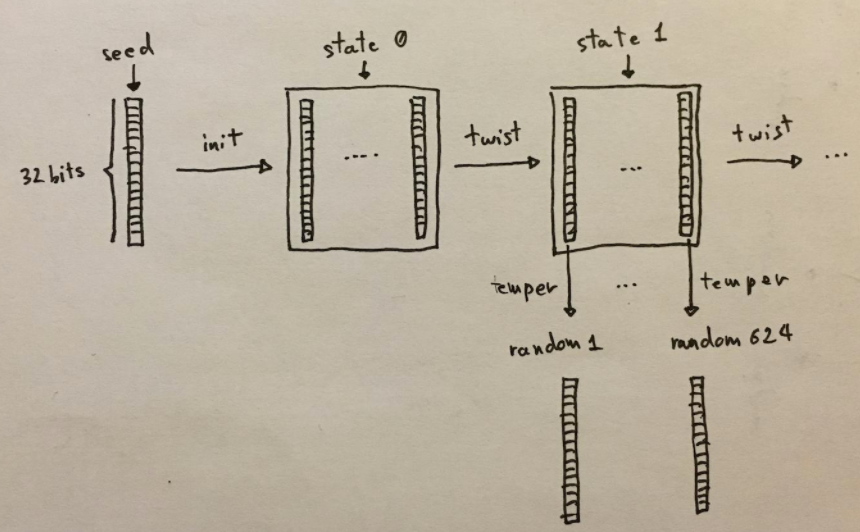
\includegraphics[width = 0.6\textwidth]{figure_man/mersenne.png} \\
\begin{footnotesize}
\url{https://www.cryptologie.net/article/331/how-does-the-mersennes-twister-work/}
\end{footnotesize}
\end{center}


\framebreak

\begin{small}
	\textbf{Note:} Here, random numbers $x_i$ are represented by $w$-bit vectors (usually $w = 32, 64$). To emphasize this, we write $\mathbf{x}_i$ (in bold).
\end{small}

\vspace*{0.2cm}

\textbf{Description of the algorithm:}
\begin{enumerate}
\item \textbf{Initialization: } A seed $\mathbf{x}_0$ is set, and the first $n$ values are calculated based on it (not described here). These values are not part of the final output.
\vspace*{0.2cm}
\begin{center}
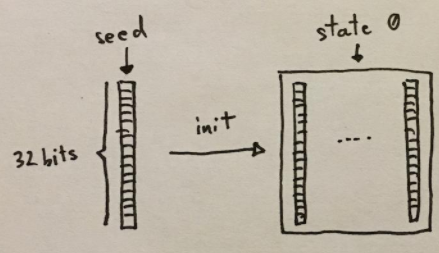
\includegraphics[width = 0.6\textwidth]{figure_man/mersenneinit.png}
\end{center}

\framebreak

\item \textbf{Recursion:} Formally the following recursion formula is used

$$
\mathbf{x}_{k + n} = \mathbf{x}_{k + m}\ \underbrace{\bigoplus}_{3.}\ \underbrace{(\mathbf{x}_{k}^l ||  \mathbf{x}_{k + 1}^r)}_{1.}\ \underbrace{\mathbf{A}}_{2.}
$$

\begin{itemize}
	\item $n$: Degree of recurrence, "size" of blocks
	\item $m$: Integer $1 \le m < n$
	\item $\mathbf{x}_{k}^l$, $\mathbf{x}_{k}^r$: Left and right part of the vector $x_{k}$
	\item $0 \le c \le w - $1 determines where the "left part" ends
\end{itemize}

\vspace*{0.2cm}

\begin{center}
	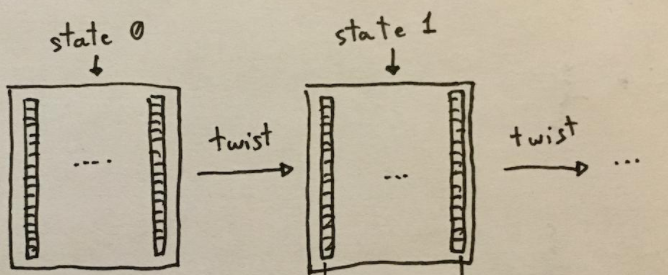
\includegraphics[width = 0.5 \textwidth]{figure_man/twist.png}
\end{center}

\framebreak

For ease of exposition, let $w = 4$, $c = 2$.

\lz

\textbf{1. Concatenation:}

$$
\begin{array}{r} \mathbf{x}_k \\ \mathbf{x}_{k + 1} \\ \mathbf{x}_{k + 2} \end{array}\begin{pmatrix} \textcolor{green}{0} & \textcolor{green}{1} & 1 & 0 \\
\textcolor{red}{1} & \textcolor{red}{0} & \textcolor{green}{1} & \textcolor{green}{0} \\
1 & 1 & \textcolor{red}{1} & \textcolor{red}{1}
\end{pmatrix} \Rightarrow \begin{matrix}
(x_{k}^l || x_{k + 1}^r) & = (\textcolor{green}{0}, \textcolor{green}{1}, \textcolor{green}{1}, \textcolor{green}{0}) \\
(x_{k + 1}^l || x_{k + 2}^r) & = (\textcolor{red}{1}, \textcolor{red}{0}, \textcolor{red}{1}, \textcolor{red}{1})
\end{matrix}
$$

\framebreak
\begin{footnotesize}
\textbf{2. Multiplication by $\mathbf{A}$: }


We multiply with the so-called \textbf{Twist Matrix} $\mathbf{A}$

$$
\mathbf{A} = \begin{pmatrix}
0 & 1 & 0 & 0  \\
0 & 0 & 1 & 0 \\
 0 & 0 & 0 & 1 \\
a_{3} & a_{2} & a_{1} & a_0
\end{pmatrix}
$$

\begin{eqnarray*}
(0, 1, 1, 0)  \mathbf{A} &=& (0, 0, 1, 1)\\
(1, 0, 1, 1) \mathbf{A} &=& (0 \oplus a_3, 1 \oplus + a_2, 0 \oplus a_1, 1 \oplus a_0)
\end{eqnarray*}

In summary $\quad
\mathbf{x}\mathbf{A} = \begin{cases}
\text{shift}(\mathbf{x}), \quad \text{if last bit } x_0 = 0 \\
\text{shift}(\mathbf{x}) \oplus \mathbf{a} , \quad \text{if } x_0 = 1
\end{cases}
$

%\framebreak
\lz

\textbf{3. XOR: }


In the last step a bitwise XOR is calculated, e.g.

$$
\mathbf{x}_{k + m} \bigoplus (0, 0, 1, 1)
$$
\end{footnotesize}

\framebreak

\item \textbf{Tempering:}  In the last step, tempering is applied to the generated random numbers in order to improve their distribution properties.

\vspace*{0.2cm}

\begin{center}
	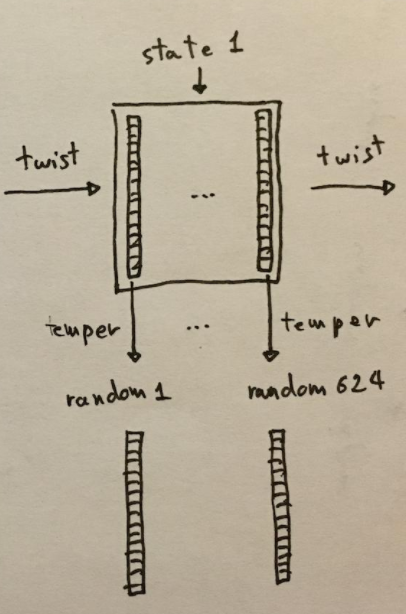
\includegraphics[width = 0.3 \textwidth]{figure_man/temper.png}
\end{center}
\end{enumerate}

\framebreak

The following operations are performed:
\vspace*{-0.2cm}
\begin{eqnarray*}
\mathbf{x} &\mapsto& \mathbf{y} := \mathbf{x} \oplus ((\mathbf{x} >> u) \text{ AND } \mathbf{d}) \\ \mathbf{y} &\mapsto& \mathbf{y} := \mathbf{y} \oplus ((\mathbf{y} << s) \text{ AND } \mathbf{b}) \\
\mathbf{y} &\mapsto& \mathbf{y} := \mathbf{y} \oplus ((\mathbf{y} < < t) \text{ AND } \mathbf{c}) \\ \mathbf{y} &\mapsto& \mathbf{z} := \mathbf{y} \oplus (\mathbf{y} >> l)
\end{eqnarray*}

where $\mathbf{x} >> u$ ($\mathbf{x} << u$) describes the bitwise "right"-shift ("left"-shift) by $u$ and "AND" describes the bitwise "and".

\lz

This can be summarized as follows:

$$\mathbf{x} \mapsto \mathbf{z} = \mathbf{x}\mathbf{T}. $$


\framebreak

Coefficients for MT19937: (standard implementation 32-bit)

\begin{description}
  \item[w] word size (in number of bits): 32
  \item[n] degree of recurrence: 624
  \item[m] middle word, an offset used in the recurrence relation defining the series x: 397
  \item[c] separation point of one word, or the number of bits of the lower bitmask: 31
  \item[a] coefficients of the rational normal form twist matrix: $9908B0DF_{16}$
  \item[u, d, l] tempering masks/shifts: $(11, FFFFFFFF_{16}, 18)$
  \item[s, b] tempering masks/shifts: $(7, 9D2C5680_{16})$
  \item[t, c] tempering masks/shifts:  $(15, EFC60000_{16})$
\end{description}

\framebreak


\textbf{Properties}:

\begin{itemize}
	\item Extremely long period of $2^{19937} - 1\approx 4.3 \cdot 10^{6001}$ (so-called "Mersenne prime")
	\item All bits of the output sequence are uniformly distributed $\to$ thus the corresponding integer values are also uniformly distributed
	\item Low correlation of consecutive values
	\item Fast implementation by calculating $n$ ($n = 624$ in MT19937) random numbers in one step
	\item Highly parallelizable
\end{itemize}

\lz

\footnotesize{
Further information:
\begin{itemize}
	\item \url{www.math.sci.hiroshima-u.ac.jp/~m-mat/MT/ARTICLES/mt.pdf} (Original paper Mersenne Twister)
	\item \url{http://statweb.stanford.edu/~owen/mc/Ch-unifrng.pdf} (Lecture on PRNGs)
\end{itemize}
}
% https://bugs.r-project.org/bugzilla/show_bug.cgi?id=17494

\end{vbframe}


% \subsection{Shift Register Methoden}


% \begin{vbframe}{Twisting / Shuffling}
% Multiplikative und lineare Kongruenzgeneratoren haben zu hohe
% Autokorrelation, insbesondere sind $n$-Tupel nicht gleichverteilt im
% $n$-dimensionalen Einheitswürfel, sondern konzentrieren sich nahe
% weniger Hyperebenen.\\
% \medskip
% Eine einfache Möglichkeit, um zumindest Tupel der Länge $n$ ohne
% Autokorrelation zu bekommen, ist diese automatisch zu mischen.
% \begin{enumerate}
%  \item Initialisiere $s_i=u_i$, $i=1,\ldots,n$, und $y=s_n$.
%  \item Erzeuge neuen Wert $u$, setze $j=\lceil y \cdot n \rceil$.
%  \item Setze $y=s_j$ und $s_j=u$.
%  \item Gib Zufallszahl $y$ zurück, wiederhole ab 2.
% \end{enumerate}
% $u_i$ aus einem Standardgenerator, Seed sind die $n$ Zahlen $s_n$.
%
% \framebreak
%
% <<echo=FALSE>>=
% shuffle = function(n, rand = mkg, ...) {
%   u = mkg(n * 2, ...)
%   s = u[1:n]
%   k = n
%   x = NULL
%   for(i in 1:n) {
%     j = as.integer(s[k] * k) + 1
%     x = c(x, s[k])
%     s[k] = s[j]
%     s[j] = u[n + i - 1]
%   }
%   return(x)
% }
% @
%
% <<echo=FALSE>>=
% randu = shuffle(12000, 1, m = 2^31, a = 2^16 + 3)
% randu3D = as.data.frame(matrix(randu, ncol = 3, byrow = TRUE))
% colnames(randu3D) = c("x1", "x2", "x3")
% @
%
% <<echo=FALSE, rgl=TRUE>>=
% library("rgl")
% mfrow3d(1, 3)
% with(randu3D, plot3d(x1, x2, x3))
% rgl.viewpoint(theta = -12.8, phi = 3.3, fov = 0, zoom = 0.7)
% with(randu3D, plot3d(x1, x2, x3))
% rgl.viewpoint(theta = -6.8, phi = 3.3, fov = 0, zoom = 0.7)
% with(randu3D, plot3d(x1, x2, x3))
% rgl.viewpoint(theta = -3.8, phi = 3.8, fov = 0, zoom = 0.7)
% @
%
% {\footnotesize \emph{Hinweis:} Erneut der selbe Plot
% aus drei verschiedenen Perspektiven.}
%
% % <<>>=
% % z = with(randu, (6 * x2 - 9 * x1) %% 1)
% % head(cbind(z, randu$x3))
% % @
% \end{vbframe}
%
%
% \begin{fragileframe}{Shift-Register-Methode}
% \textbf{Grundlage:} Bei der Shift-Register-Methode wird eine Bitfolge X
% durch Rekursion erzeugt. Für das Element n der Folge gilt:
% $$
% X_n = X_{n-p} \oplus  X_{n-p + q}, \quad 1 < q < p,
% $$
% wobei $\oplus$ für exklusives Oder steht:
%
% \lz
%
% \begin{table}
% \centering
% \begin{tabular}{|cc|c|}
%   \hline
% $X_{n-p}$ & $X_{n-p + q}$  & $X_n$ \\
%   \hline
% \textcolor{green}{0} & \textcolor{green}{0} & \textcolor{red}{0} \\
% \textcolor{green}{0} & \textcolor{green}{1} & \textcolor{red}{1} \\
% \textcolor{green}{1} & \textcolor{green}{0} & \textcolor{red}{1} \\
% \textcolor{green}{1} & \textcolor{green}{1} & \textcolor{red}{0} \\
%    \hline
% \end{tabular}
% \end{table}
%
% Es wird eine Startfolge der Länge p benötigt.
%
%
% <<include=FALSE>>=
% source("rsrc/ieee754.R")
% as.dec.bin("1011")
% as.bin(11)
% as.dec(as.bin(11))
% @
%
% \framebreak
%
% <<echo=FALSE>>=
% shift = function(n, seed = 11, bits = 4, p = 4, q = 3) {
%   x = as.bin(seed, unsigned = TRUE)
%   x = as.integer(strsplit(x, "")[[1]])
%   k = length(x)
%   for(i in 1:(n * bits)) {
%     x = c(x, as.integer(xor(x[k - p + 1], x[k - p + q + 1])))
%     k = length(x)
%   }
%   i = split(1:k, ceiling(seq_along(1:k) / bits))
%   x = as.character(sapply(i, function(j) {
%     paste(x[j], collapse = "")
%   }))
%   x = sapply(x, function(b) {
%     if(nchar(b) < bits) {
%       b = paste(b, paste(rep(0, bits - nchar(b)),
%         collapse = ""),
%       sep = "")
%     }
%     b
%   })
%   ix = sapply(x, as.dec.bin)
%   rval = data.frame(
%     "bin" = x,
%     "int" = ix,
%     "u" = ix / (2^bits),
%     stringsAsFactors = FALSE
%   )
%   rval
% }
% @
%
% % <<eval=FALSE>>=
% % shift = function(n, seed = 11, bits = 4, p = 4, q = 3) {
% %   x = as.bin(seed, unsigned = TRUE)
% %   x = as.integer(strsplit(x, "")[[1]])
% %   k = length(x)
% %   for(i in 1:(n * bits)) {
% %     x = c(x, as.integer(xor(x[k - p + 1], x[k - p + q + 1])))
% %     k = length(x)
% %   }
% %   i = split(1:k, ceiling(seq_along(1:k) / bits))
% %   x = as.character(sapply(i, function(j) {
% %     paste(x[j], collapse = "")
% %   }))
% % @
%
% % <<eval=FALSE>>=
% %   x = sapply(x, function(b) {
% %     if(nchar(b) < bits) {
% %       b = paste(b, paste(rep(0, bits - nchar(b)),
% %         collapse = ""),
% %       sep = "")
% %     }
% %     b
% %   })
% %   ix = sapply(x, as.dec.bin)
% %   rval = data.frame(
% %     "bin" = x,
% %     "int" = ix,
% %     "u" = ix / (2^bits),
% %     stringsAsFactors = FALSE
% %   )
% %   rval
% % }
% % @
%
%
% \textbf{Beispiel:} $p = 4, q = 3$, Startfolge: $1011$.
%
% \begin{footnotesize}
%
% \begin{eqnarray*}
% X_5 &=& X_{1} \oplus  X_{4} = 1 \oplus 1 = 0 \\
% X_6 &=& X_{2} \oplus  X_{5} = 0 \oplus 0 = 0 \\
% X_7 &=& X_{3} \oplus  X_{6} = 1 \oplus 0 = 1 \\
%     &\hdots&
% \end{eqnarray*}
%
% \begin{table}
% \begin{tabular}{rrrrrrrrrr}
%   \hline
%   &   &   & \textcolor{green}{1} & 0 & 1 & 1 & & & \\
%   \hline
% 1 & 0 & 1 & \textcolor{green}{1} & \textcolor{red}{0} & & & & \\
%   \hline
%   \hline
%   &   &   & 1 & \textcolor{green}{0} & 1 & 1 & 0 & &\\
%   \hline
% 1 & 0 & 1 & 1 & \textcolor{green}{0} & \textcolor{red}{0} & & & &\\
%   \hline
%   \hline
%   &   &   & 1 & 0 & \textcolor{green}{1} & 1 & 0 & 0 &\\
%   \hline
% 1 & 0 & 1 & 1 & 0 & \textcolor{green}{0} & \textcolor{red}{1} & & &\\
%   \hline
%   \hline
%   &   &   & 1 & 0 & 1 & \textcolor{green}{1} & 0 & 0 & 1\\
%   \hline
% 1 & 0 & 1 & 1 & 0 & 0 & \textcolor{green}{1} & \textcolor{red}{0} & & \\
%   \hline
% \end{tabular}
% \end{table}
%
% \end{footnotesize}
% \framebreak
%
% <<size="scriptsize">>=
% shift(15)
% @
%
% \framebreak
%
% Im Beispiel codieren Vierergruppen Integer zwischen 1 und 15
% $$
% \text{Zufallszahlen} \quad y_i = \sum\limits_{j=1}^4 2^{-j} X_{4i+j}
% $$
% Periode der Länge $15 = 2^4 - 1$
% (gilt auch für Bits).
% Im Allgemeinen muss nicht gelten, dass Gruppenlänge $M = p$.\\
% \bigskip
% Wahl der Parameter nicht egal. Wähle oben $q = 2$:
%
% <<>>=
% shift(3, q = 2)
% @
%
% \framebreak
%
% Für $q = 1$ und $p = 5$ und Bitlänge 5, erhält man auch nur Periode der Länge 3:
%
% <<>>=
% shift(9, seed = 22, q = 1, p = 5, bits = 5)
% @
% \end{fragileframe}
%
%
% \begin{vbframe}{Generalized Feedback Shift Register (GFSR)}
% Lewis und Payne (1973):
% $$
% y_i = \sum\limits_{j=1}^M 2^{-j} X_{i-s(j)}
% $$
% Typisch: $s(1)=0 < s(2) < \dots < s(M)$ \\
% Ursprünglicher Vorschlag: $s(j) = 100 p (j-1)$, mit $p = 98$ und $q = 27$.
% \begin{itemize}
% \item Liefert große Integer mit langen Perioden $(2^p-1)$.
% \item unabhängig von Maschinenarithmetik (brauche nur $\oplus$)
% \item hervorragende multivariate Eigenschaften
% \end{itemize}
% {\bf Größter Nachteil:}  Nicht triviale Initialisierung. \\
% Benötige Startsequenz der Länge $p$ und nicht jede Startsequenz garantiert optimale Eigenschaften (vgl. Monahan).
% \end{vbframe}
%
%
% \begin{vbframe}{Mersenne-Twister}
% Bei GSFR gilt Rekurrenzrelation für alle Komponenten der Vektoren\\
% $Y_n = [X_n, X_{n - s(2)}, \dots,  X_{n - s(m)}]$.
%
% \lz
%
% {\bf Twisted GFSR}: Variation der Rekursion zu
% $$
% Y_{n+p} = Y_n\ \bigoplus\ (Y_{n+q}^l, Y_{n+q+1}^r)\ \mathbf{A},
% $$
% wobei $Y_{n}^l$ die erste Hälfte und $Y_{n}^r$ die zweite Hälfte
% der Bits und $\mathbf{A}$ eine geeignete Matrix
%
% \lz
%
% {\bf Mersenne-Twister}: Matsumoto und Nishimura (1998),\\
% $p = 624$, $q = 397$, Matrix $\mathbf{A}$ erzeugt nur einfache Bit-Shifts.
% \end{vbframe}


\begin{vbframe}{Transformation to the Interval $(0, 1)$}

\vspace*{-0.4cm}

\begin{itemize}
\item In the procedures discussed, integers between $0$ and $m - 1$ were generated.
\item If real random numbers in the interval $(0, 1)$ need to be simulated, a simple division by $m$ is sufficient.
\item \textbf{Problem:} The random number can be $0$, while for an "actual" $(0, 1)$ - uniformly distributed random variable $U$ the following holds:
$$
\mathbb{P}(U = 0) = 0
$$
\item This is often a problem in practical applications, e.g. with $\log(U)$.
\item If a $0$ is generated, the random number can be discarded or an error message is issued.
\item Since modern congruential generators have a long period, this is unlikely.
\end{itemize}
%
% \begin{table}
% \begin{footnotesize}
% \centering
% \begin{tabular}{r|rrrrrrrrrr}
%   \hline
%  i & 1 & 2 & 3 & 4 & 5 & 6 & 7 & 8 & 9 & 10 \\
%   \hline
% 0  & 0.29 & 0.94 & 0.41 & 0.12 & 0.18 & 0.76 & 0.65 & 0.47 & 0.71 & 0.06 \\
% 10 & 0.59 & 0.88 & 0.82 & 0.24 & 0.35 & 0.53 & 0.29 & 0.94 & 0.41 & 0.12 \\
% 20 & 0.18 & 0.76 & 0.65 & 0.47 & 0.71 & 0.06 & 0.59 & 0.88 & 0.82 & 0.24 \\
% 30 & 0.35 & 0.53 & 0.29 & 0.94 & 0.41 & 0.12 & 0.18 & 0.76 & 0.65 & \ldots \\
%    \hline
% \end{tabular}
% \end{footnotesize}
% \end{table}

\end{vbframe}

\begin{vbframe}{PRNGs in \texttt{R}}
The Mersenne Twister is (currently) the default method in \texttt{R} with period
$2^{19937} - 1 \approx 10^{6001}$ and guaranteed uniform distribution in
623 dimensions.
Seeds are 624 32-bit integers on top of the current position in this set. The \code{set.seed()} function generates a valid seed from a
single integer value using the linear congruential generator with
$$
  m=2^{32}, \qquad a=69069, \qquad b=1
$$
There are a number of other generators available. Furthermore, the
user can also specify her own generator as default.
\code{RNGversion('x.y.z')} can be used to set the random generators as they were in an earlier \texttt{R} version (for reproducibility) (Wichman-Hill up to 0.98, Marsaglia-Multicarry up to 0.00).
1.6.1). Initialization of the seed via time.
\end{vbframe}


\begin{vbframe}{R: Random Number Generation}
\begin{itemize}
%\begin{footnotesize}
\item \code{set.seed()} function

\footnotesize
\begin{verbatim}
set.seed(123); u1 <- runif(100)
set.seed(123); u2 <- runif(100) 
identical(u1, u2) # the same because of identical RNG status
## [1] TRUE
\end{verbatim}


\normalsize
\item \code{.Random.seed()} is an integer vector, containing the random number generator (RNG) state for random number generation in \texttt{R}. It can be saved and restored, but should not be altered by the user.

\item \code{RNGkind()} is a more friendly interface to query or set the kind of RNG in use.
\footnotesize

\begin{verbatim}
# default for "kind", "normal kind" and "sample kind" 
RNGkind("default") 
RNGkind()
## [1] "Mersenne-Twister" "Inversion"  "Rejection"
.Random.seed[1:3] # the default random seed is 626 integers
## [1] 10403 624 1858651209
\end{verbatim}


\normalsize
\framebreak
\item Change default of kind ("Mersenne-Twister") to "Wichmann-Hill"

\footnotesize
\begin{verbatim}
RNGkind("Wich")
RNGkind()
## [1] "Wichmann-Hill" "Inversion" "Rejection"
.Random.seed
## [1] 10400  5989  8337  9843
\end{verbatim}


\normalsize
\item Change methods depending on defaults in a specific \texttt{R} Version

\footnotesize
\begin{verbatim}
RNGversion(getRversion()) # current version
RNGkind()
## [1] "Mersenne-Twister" "Inversion" "Rejection"
RNGversion("1.0.0") # first \texttt{R} version
## Warning in RNGkind("Marsaglia-Multicarry", "Buggy
Kinderman-Ramage", "Rounding"): buggy version of 
Kinderman-Ramage generator used
## Warning in RNGkind("Marsaglia-Multicarry", "Buggy
Kinderman-Ramage", "Rounding"): non-uniform 'Rounding' 
sampler used
\end{verbatim}


%\end{footnotesize}
\end{itemize}
\end{vbframe}





\begin{vbframe}{Parallel computing}
A complex topic is the application of random number generators for parallel computing, where a long calculation is split between several machines and processed in parallel.
Usually, a "master" distributes the jobs to several "slaves".
Initialization of seed using the two "standard" methods
\begin{itemize}
  \item Time of day or
  \item Fixed given number
\end{itemize}
is not useful.
Special algorithms for this purpose are provided e.g. in the \texttt{R} packages \pkg{rlecuyer} or
\pkg{rstreams} (both use the same algorithm from L'Ecuyer).
\end{vbframe}



\endlecture


\end{document}